The \textit{Game} module is responsible for gamification part of the system. Registered user will be able to collect points and compete with other registered users. The scope of the \textit{Game} module is shown in Figure 5.  \\[1cm]

\begin{figure}[h]
	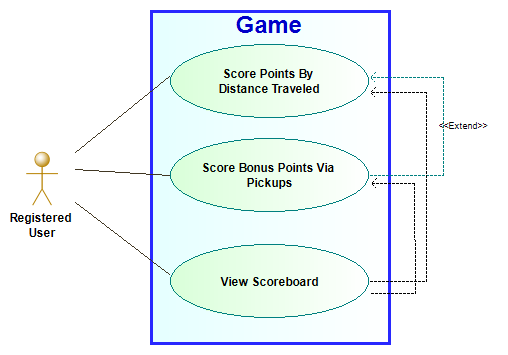
\includegraphics[width=\textwidth]{Game_Use_Case_Diagram}
	\caption{Game module use case}
\end{figure}

\begin{enumerate}
	\item \textbf{Score Points by Distance Travelled}
	\begin{itemize}
		\item Description: \\
		Allows users to score points based on their distance travelled.
		\item Pre-Conditions: \\
		\begin{itemize}
		\item User must be logged in
		
		\end{itemize}
		
		\item Post-Conditions: \\
	
	\end{itemize}
	
	\item \textbf{Score Bonus Points via Pick-ups}
	\begin{itemize}
		\item Description: \\
		Allows users to score points bases on the route travelled
		\item Pre-Conditions: \\
		\begin{itemize}
		\item User must be logged in
		
		\end{itemize}
		
		\item Post-Conditions: \\
	
	\end{itemize}
	
	\item \textbf{View Scoreboard}
	\begin{itemize}
		\item Description: \\
		Allows the user to view their scores
		\item Pre-Conditions: \\
		\begin{itemize}
		\item User must be logged in		
		\end{itemize}
		\item Post-Conditions: \\
	
	\end{itemize}
	
	
\end{enumerate}